% 16. Formato de Tablas y Figuras; 23. Política de Integridad Académica.
% Insertar en apéndices sólo al integrar el artículo; capturas originales del usuario.
\section{Evidencias de la competencia externa de Othello}
\begin{figure}[!htbp]
\centering
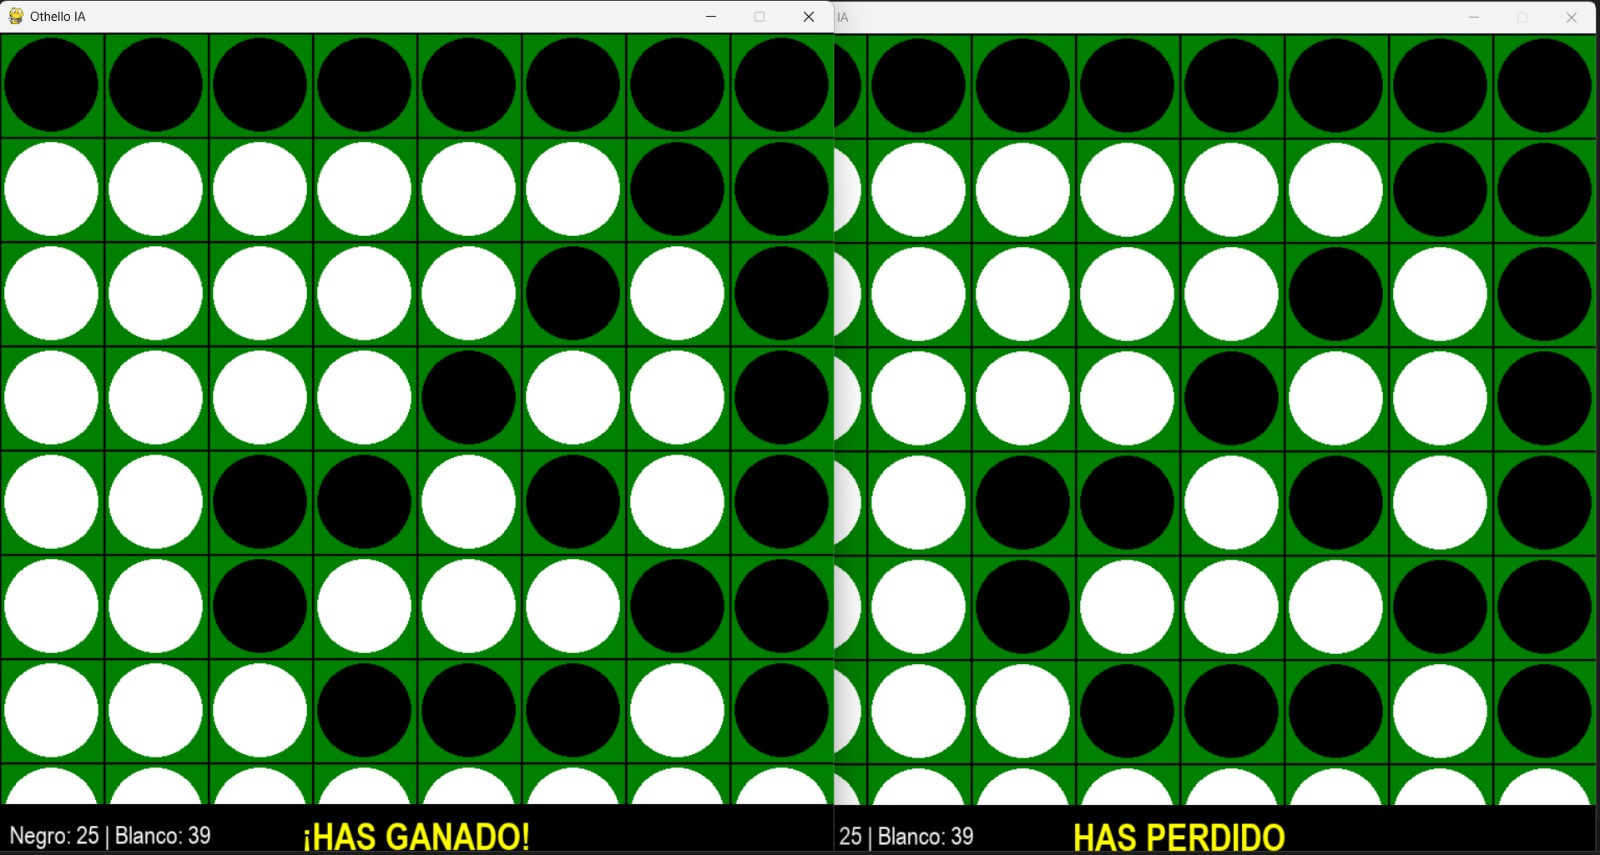
\includegraphics[width=.95\linewidth]{../datos/othello/competencia_externa/evidencias/partida-1.jpeg}
\caption{Partida 1 contra el equipo Juan Pablo. Contador negras--blancas: 25--39; Ispis jugó con negras según el reporte del usuario. Captura original sin editar; no acredita la secuencia de jugadas ni la configuración rival.}
\label{fig:othello_externa_1}
\end{figure}
\begin{figure}[!htbp]
\centering
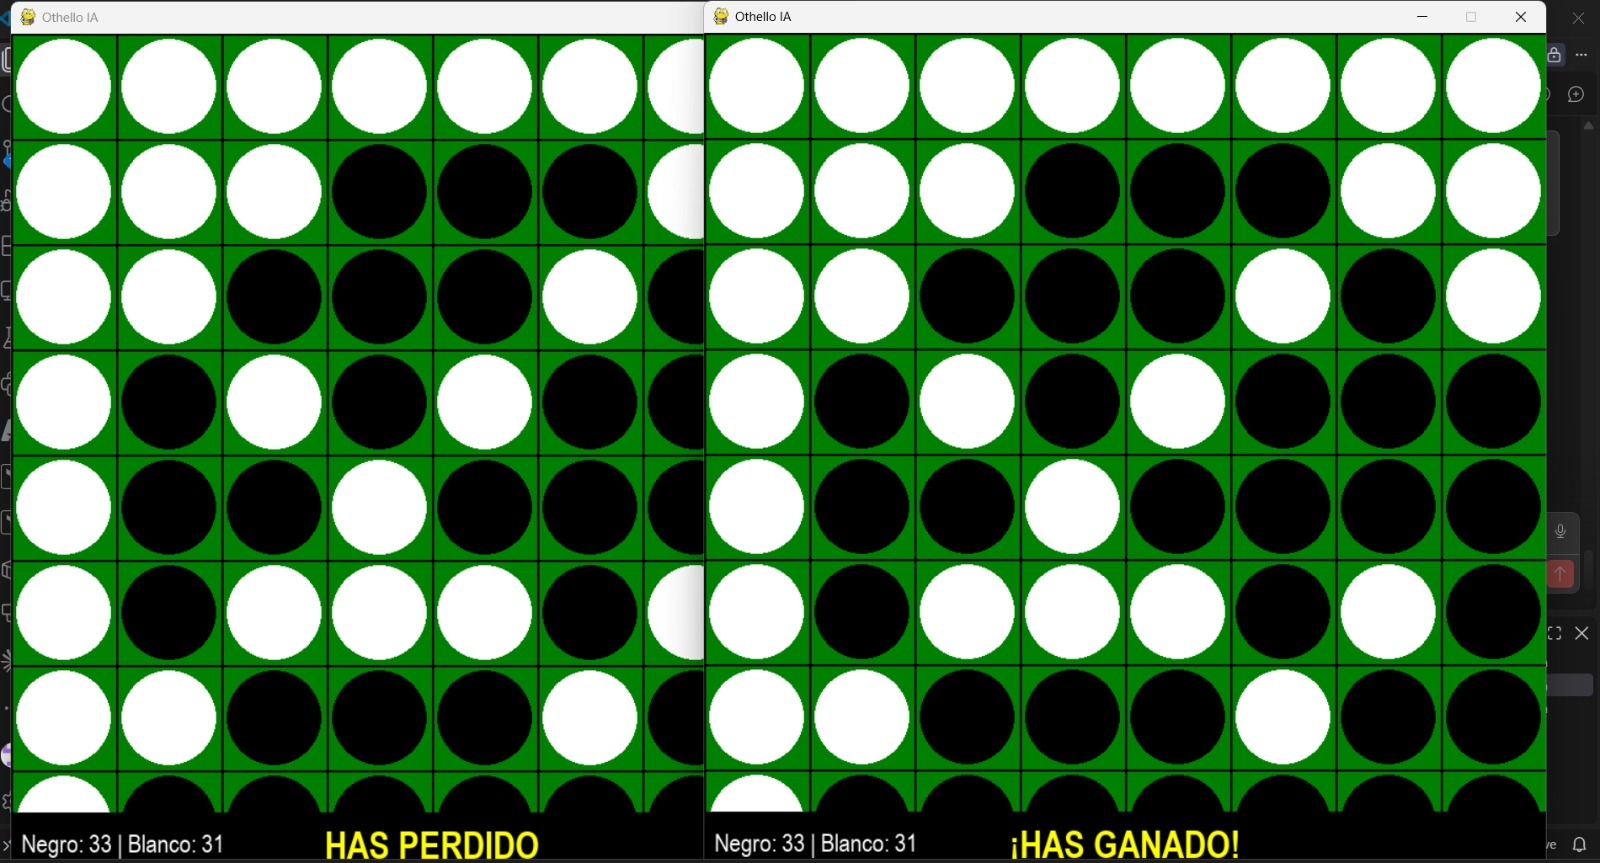
\includegraphics[width=.95\linewidth]{../datos/othello/competencia_externa/evidencias/partida-2.jpeg}
\caption{Partida 2 contra el equipo Juan Pablo. Contador negras--blancas: 33--31; Ispis jugó con blancas según el reporte del usuario. Captura original sin editar; no acredita la secuencia de jugadas ni la configuración rival.}
\label{fig:othello_externa_2}
\end{figure}
\begin{figure}[!htbp]
\centering
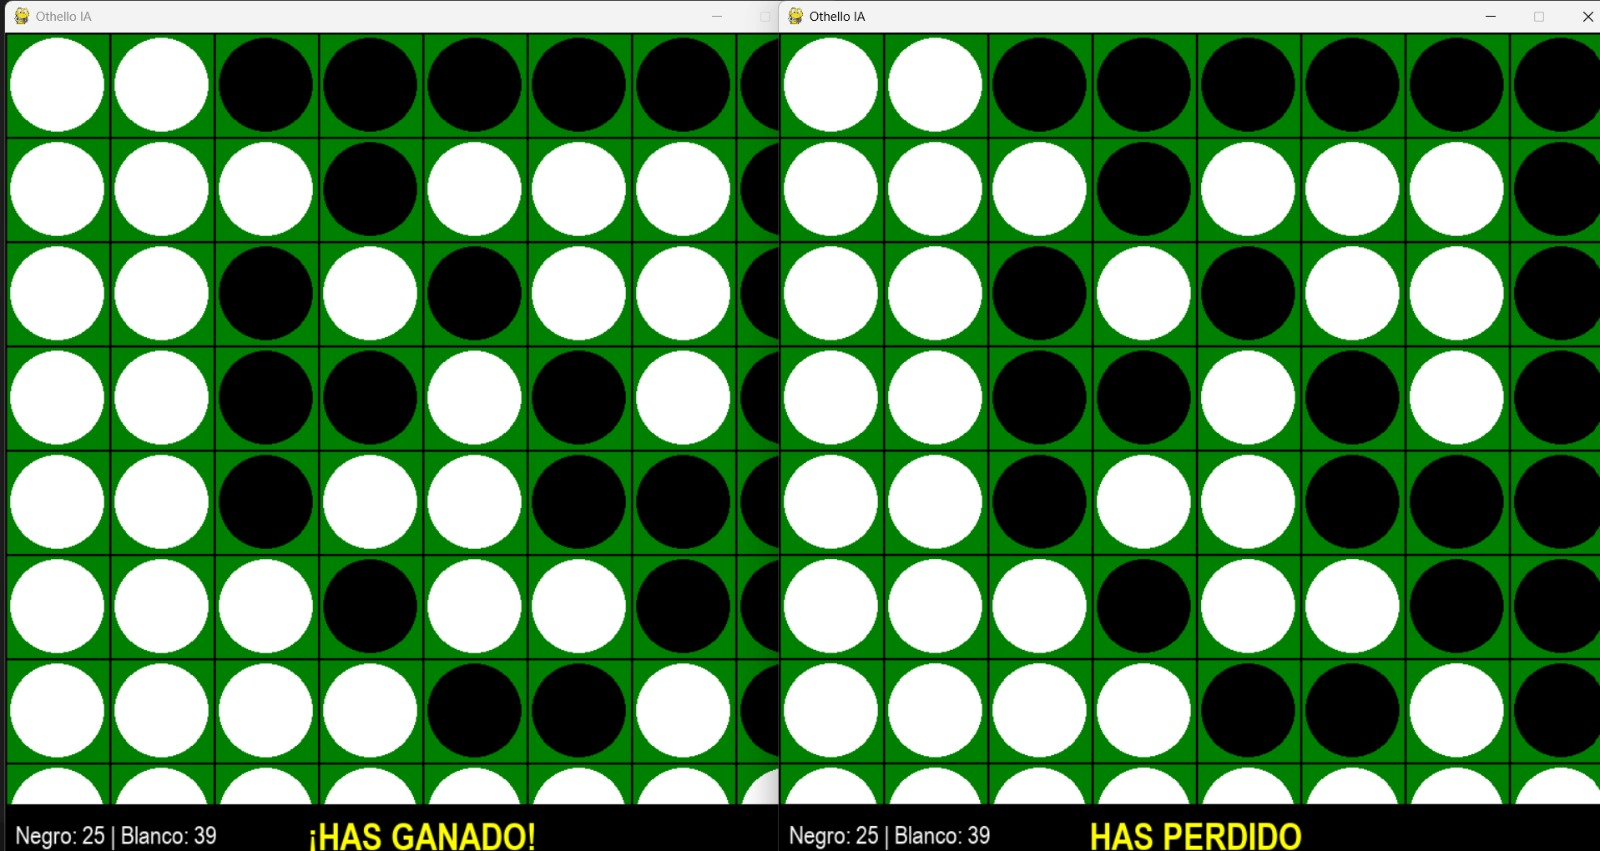
\includegraphics[width=.95\linewidth]{../datos/othello/competencia_externa/evidencias/partida-3.jpeg}
\caption{Partida 3 contra el equipo Juan Pablo. Contador negras--blancas: 25--39; Ispis jugó con negras según el reporte del usuario. Captura original sin editar; no acredita la secuencia de jugadas ni la configuración rival.}
\label{fig:othello_externa_3}
\end{figure}
